\documentclass[12pt]{article}
\usepackage{geometry}
\usepackage{amsmath}
\usepackage{amssymb}
\usepackage{enumitem}
\usepackage{fancyhdr}
\usepackage{tikz}
\usepackage{graphicx}
\usepackage{xcolor}
\usepackage{subcaption}
\usepackage{float}

\usetikzlibrary{trees}
\pagestyle{fancy}


% \lhead{Problem \arabic{enumi}}
\lhead{Jaykumar Patel}
\chead{Homework 1}
\rhead{EID: jnp2369}

\begin{document}

\title{Homework 1 Solutions}

Collaborators: Aniketh Devarasetty, Janvi Patel, Boting Lu

\section{Image Pyramids}

\subsection{Design Decisions: Gaussian and Laplacian Pyramids}
\begin{itemize}
    \item For Gaussian blurring, I used a 5x5 kernel with $\sigma = 1.0$. I chose $\sigma = 1.0$ because in class, we learned that typically, $\sigma = \sqrt{s/2}$ where $s$ is the downsampling rate. Since we are downsampling by a factor of 2, $\sigma = \sqrt{2/2} = 1.0$. Furthermore, we learned in class that typically, we set the filter size's half-width to be $3\sigma$. $3\sigma = 6$ but the filter should be odd so that there is a center pixel. Thus, I chose a 5x5 kernel.
    \item When scaling an image dowm, I used the cv2.INTER\_LINEAR interpolation method. I chose this method because it is a commonly used method for scaling down images. Also, it is a good balance between speed and quality. It essentially computes a weighted average of the neighboring pixels to determine the new pixel value.
\end{itemize}

\subsection{FFT Decisions}
\begin{itemize}
    \item I first compute the 2-D Fourier transform of the image.
    \item I also shift the zero frequency component to the center of the spectrum. 
    \item Finally, I compute the magnitude and then convert it to the logarithmic scale. This enhances visibility of the spectrum.
\end{itemize}

\subsection{Explain what the Laplacian and Gaussian pyramids are doing in terms of frequency.}

The Gaussian pyramid represents the blurred version of the image (by applying Gaussian filter) at different scales. Specifically, the Gaussian pyramid captures the low frequency components of the image. The Gaussian filter acts as a low pass filter by filtering out high frequencies. This can be seen in the frequency domain, where the Gaussian images have a whiter center (corresponding to higher values) and darker edges (corresponding to lower values). This shows that the Gaussian pyramid images have stronger low frequencies and weaker high frequencies. It is also noticable that there are faint white streaks (horizontal and vertical) that go through the center in the frequency domain. This makes sense because the original image has many horizontal and vertical edges.

On the other hand, the Laplacian pyramid represents the high frequency components of the image at different scales. These high frequencies capture the details of the image, such as edges and textures. Specifically, the Laplacian pyramid captures the residuals of the image by subtracting the blurred image from the pre-blurred image. The residuals capture the high frequencies of the original image. This can be seen in the frequency domain, where the Laplacian images have a darker center (corresponding to lower values) and whiter edges (corresponding to higher values). This shows that the Laplacian pyramid images (residuals) have stronger high frequencies and weaker low frequencies.

In essence, the Gaussian pyramid captures the low frequency components and smooths out fine details, while the Laplacian pyramid captures the high frequency components that are lost during the blurring process.

\begin{figure}[H]
    \centering
    \begin{subfigure}[b]{\textwidth}
        \centering
        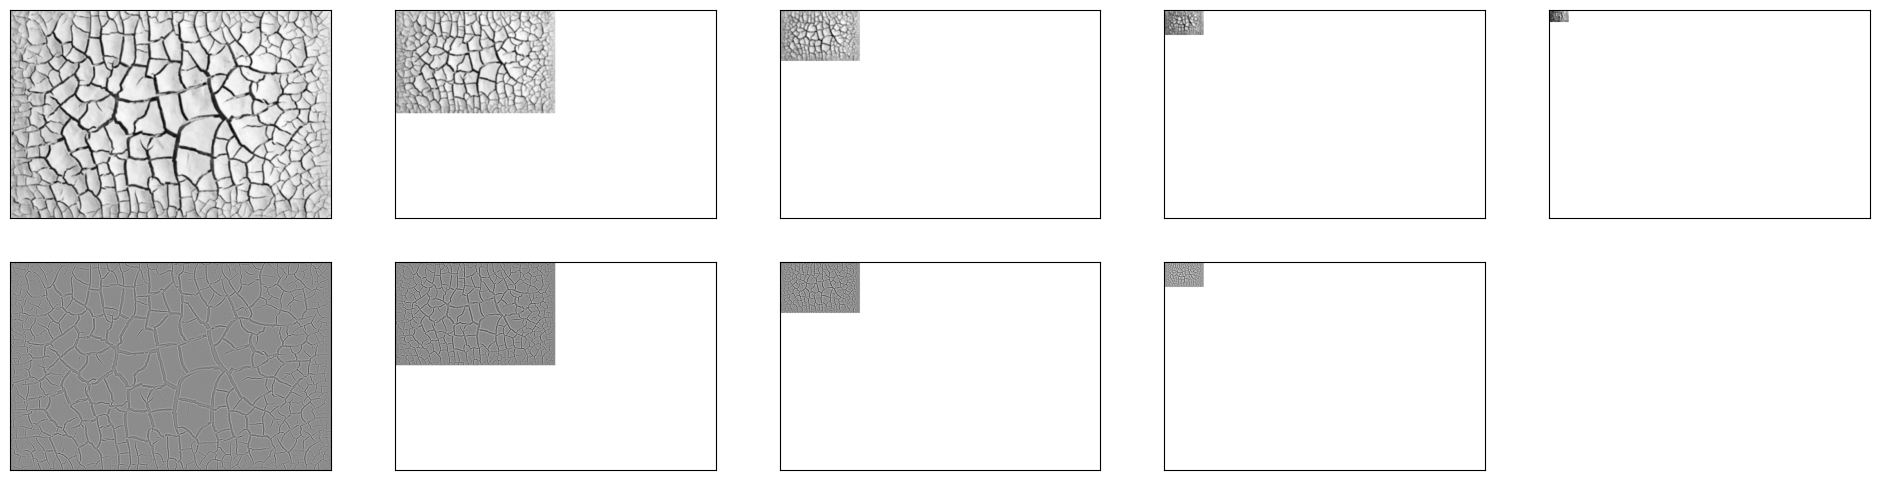
\includegraphics[width=\textwidth]{images/Gaussian_Laplacian_Pyramid.png}
        \caption{Gaussian and Laplacian Pyramids}
        \label{fig:sub1}
    \end{subfigure}
    
    \begin{subfigure}[b]{\textwidth}
        \centering
        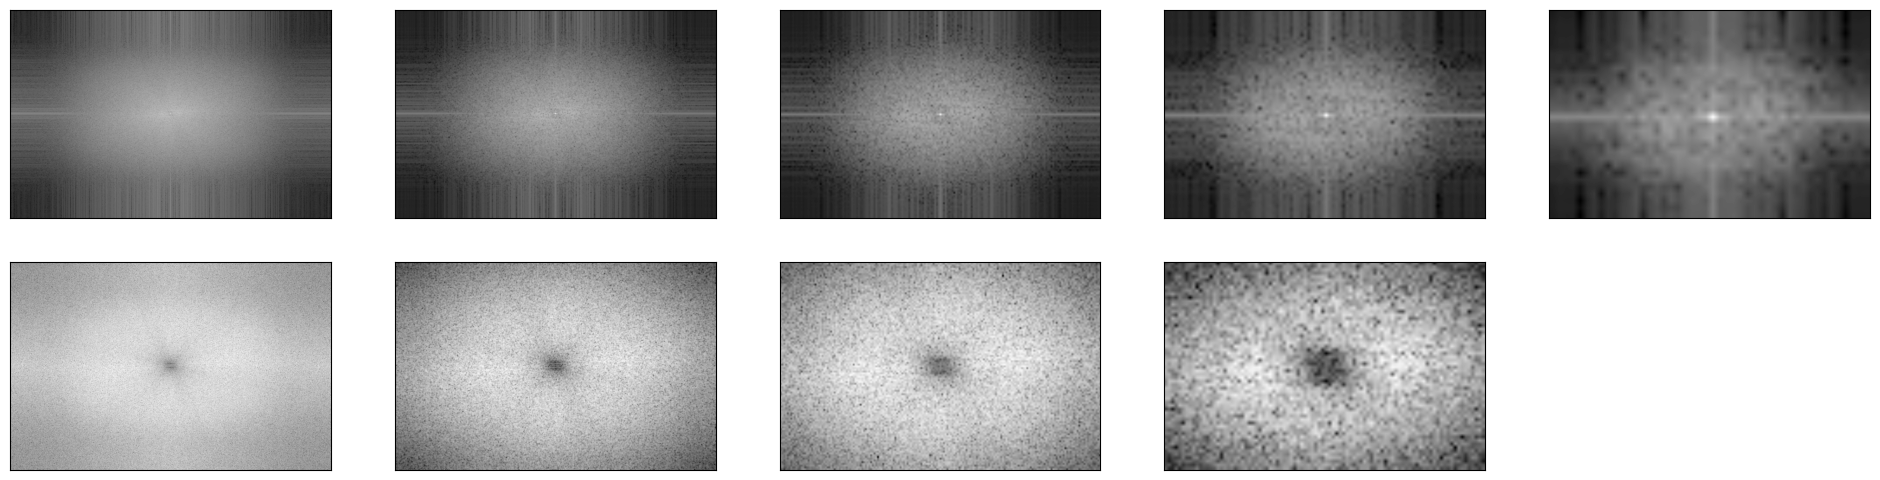
\includegraphics[width=\textwidth]{images/Gaussian_Laplacian_Frequency.png}
        \caption{Frequency Domain of Gaussian and Laplacian Pyramids}
        \label{fig:sub2}
    \end{subfigure}
    
    \caption{Pyramids and Frequency Domain}
    \label{fig:main}
\end{figure}


\section{Edge Detection}

\subsection{Design Decisions: Simple Gradient-Based Edge Detector}
\begin{itemize}
    \item I first apply a Gaussian filter to the image, using $\sigma = 1.0$ and a 5x5 kernel. I chose $\sigma = 1.0$ and a 5x5 kernel for the same reasons as in the previous section.
    \item Then I split the image into its R, G, and B channels
    \item Then, I applied the X, and Y sobel filters to each channel
    \item Then, I computed the magnitude and theta of the gradients for each channel
    \item Then, I combined the magnitudes of each channel using L2 norm to get the final magnitude.
    \item Finally, I computed the theta of the final magnitude by using the theta of the channel with the highest magnitude. I did this using the $np.argmax$ and $np.take\_along\_axis$ functions.
\end{itemize}

\subsection{Design Decisions: Oriented Filters}
\begin{itemize}
    \item Two of the filter orientations I chose were the 0 and 90 degrees. This corresponds to the traditional Sobel filter directions. I chose these because any angle can be easily represented as a combination of these two angles. 
    \item The other two filter orientations I chose were 30 and 150 degrees. Although a combination of 0 and 90 degrees can capture any degree, adding 30 and 150 degrees can help increase the edge detection sensitivity.
    \item I first apply a Gaussian filter to the image, using $\sigma = 1.0$ and a 5x5 kernel. I chose $\sigma = 1.0$ and a 5x5 kernel for the same reasons as in the previous section.
    \item Then, I split the image into its R, G, and B channels
    \item Then, I applied the 0, 30, 90, and 150 degree oriented filters to each channel
    \item Then, I computed the magnitude for each oriented filters by computing the L2 norm of oriented filter applied to the R, G, and B channels. This results in 4 magnitude matrices, one for each oriented filter.
    \item Finally, I computed the final magnitude by taking the maximum magnitude of the 4 magnitude matrices. I did this using the $np.max$ function. The final theta matrix was computed by using the orientation associated with the maximum magnitude. I did this using the $np.argmax$ and $np.take\_along\_axis$ functions.
    \item Note: the $orientedFilterMagnitude$ takes an image and a $filter\_type\_dist$ (which is a boolean) as an input. This value is used to determined how the oriented filter is created. I have implemented 2 methods of creating the oriented filter. Essentially, $getOrientedFilterUsingDistribution$ samples a 2-D distribution at certain points, whereas $getOrientedFilterUsingCombination$ uses a combination of the X and Y Sobel filters to create the oriented filter. By default, $getOrientedFilterUsingDistribution$ is used.
\end{itemize}

\subsection{Bank of Filters used for Problem 2.2}
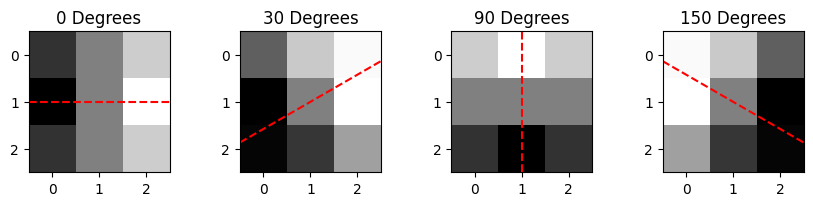
\includegraphics[width=\textwidth]{images/FiltersBank.png}


\subsection{Comparison of Detected Edges in Problem 2.1 and 2.2}
The edge detection without the non-maxima suppression look very similar for Problem 2.1 and 2.2. This makes sense since X and Y directions are sufficient to capture the gradient magnitudes, since any angle can be represented as a combination of X and Y directions. 

However the edge detection with non-maxima suppression looks different. This is because the theta matrix calculation (gradient direction calculation) is different for Problem 2.1 and 2.2, and thus, the non-maxima suppression will be different. The non-maxima suppressed image for 2.2 has thinner (and more dotted) edges than 2.1 (as shown in images below), but the edge for 2.2 is more dotted compared to 2.1. This makes sense because the theta matrix for 2.1 is calculated by combining X and Y gradients (per color channel), allowing for more angles to be represented. On the other hand, the theta for 2.2 is calculated by taking the orientation (0, 30, 90, or 150) with the highest gradient magnitude, which can result in a more limited set of angles. In other words, for 2.2, the values in the final theta matrix can only be 0, 30, 90, or 150, while for 2.1, the values can be any angle. This can result in a more limited set of angles for the non-maxima suppression for 2.2, resulting in more dotted edges as non-maxima suppression may occur at a direction different than the true direction of the gradient.

In summary, the edge detection with non-maxima suppression for 2.2 shows more dotted edges compared to 2.1. On the other hand, the edge detection without non-maxima suppression looks very similar for 2.1 and 2.2.

\begin{figure}[H]
    \centering
    \begin{subfigure}{0.45\textwidth} % Adjust the width as needed
        \centering
        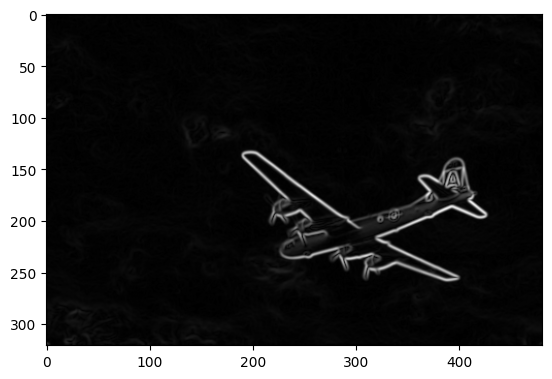
\includegraphics[width=\textwidth]{images/2_1_without_non_maxima.png}
        \caption{2.1 without non-maxima suppression}
        \label{fig:sub1}
    \end{subfigure}
    \hfill % Add horizontal space between the subfigures
    \begin{subfigure}{0.45\textwidth} % Adjust the width as needed
        \centering
        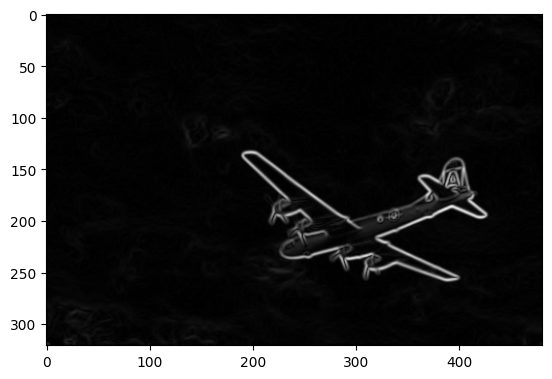
\includegraphics[width=\textwidth]{images/2_2_without_non_maxima.png}
        \caption{2.2 without non-maxima suppression}
        \label{fig:sub2}
    \end{subfigure}
    \caption{Edge detection without non-maxima suppression for 2.1 and 2.2}
    \label{fig:main}
\end{figure}


\begin{figure}[H]
    \centering
    \begin{subfigure}{0.45\textwidth} % Adjust the width as needed
        \centering
        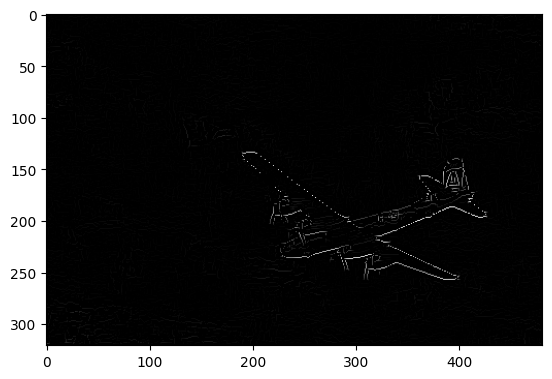
\includegraphics[width=\textwidth]{images/2_1_with_non_maxima.png}
        \caption{2.1 with non-maxima suppression}
        \label{fig:sub1}
    \end{subfigure}
    \hfill % Add horizontal space between the subfigures
    \begin{subfigure}{0.45\textwidth} % Adjust the width as needed
        \centering
        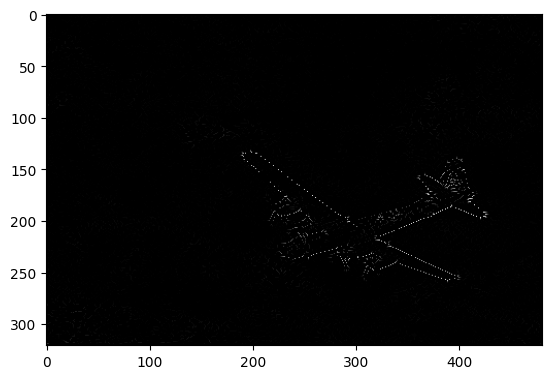
\includegraphics[width=\textwidth]{images/2_2_with_non_maxima.png}
        \caption{2.2 with non-maxima suppression}
        \label{fig:sub2}
    \end{subfigure}
    \caption{Edge detection with non-maxima suppression for 2.1 and 2.2}
    \label{fig:main}
\end{figure}


\subsection{Ideas for Improvement}
\begin{itemize}
    \item In class, we learned that 'Hysteresis' Thresholding is a part of Canny edge detector. It is useful in connecting disconnected edges, resulting in closed edges. Implementing this will improve the edge detection.
    \item For part 2.2, I chose 30 and 150 degrees as the angles for the oriented filters, in addition to 0 and 90 degrees. This selection can be improved by using PCA to find the principal directions of the edges in the image. Those princpal directions can be used to generate oriented filters. This will allow for a more accurate selection of angles for the oriented filters, and can result in a more accurate edge detection.
    \item Furthemore, using more than 4 oriented filters can improve the edge detection. Using more oriented filters can allow the edge detector to be more sensitive, potentially capturing more edges.
    \item In Canny Edge Detector we apply a gaussian filter and then apply sobel filters. This is effectively "Derivative of Gaussian". Edge detection could be potentially improved by using a "Laplacian of Gaussian" filter, which is basically a second derivative filter. This can help creating thinner edges. However, it is important to note that the non-maxima suppression in Canny Edge Detector is designed to thin the edges, so the Laplacian of Gaussian filter may not be necessary.
\end{itemize}

\end{document}